\subsection{Premi::Model}
	\begin{figure}[h]
		\centering
		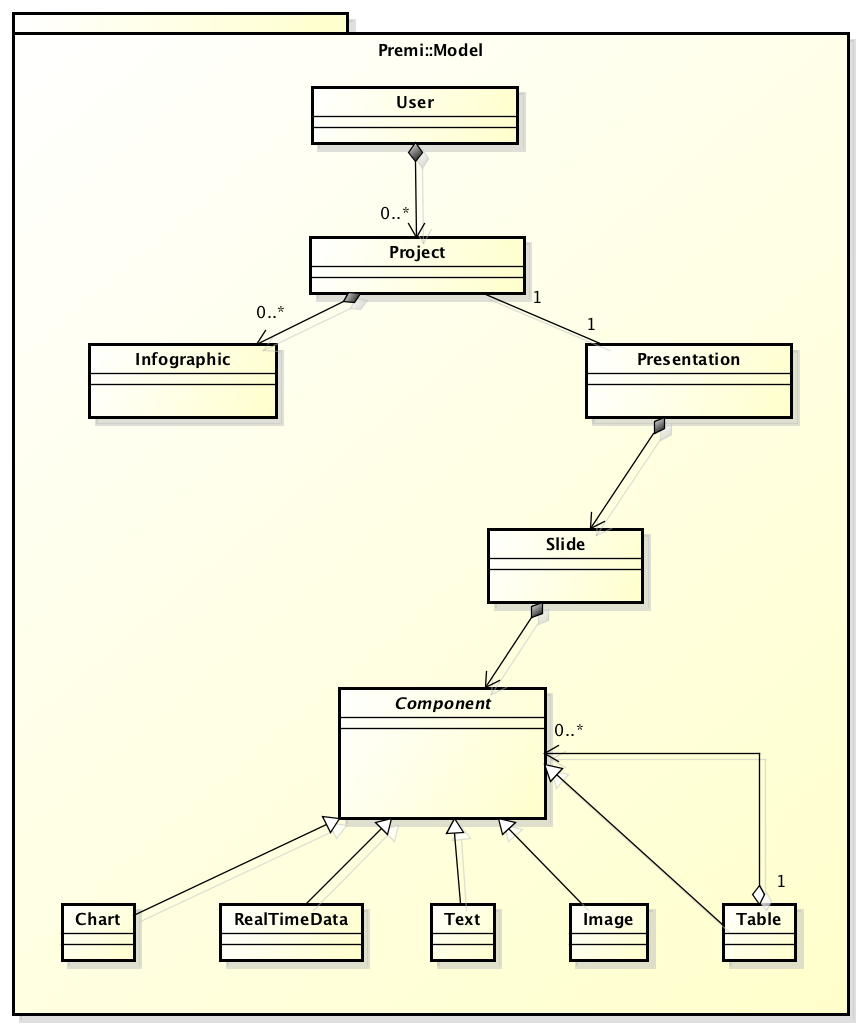
\includegraphics[width=0.7\linewidth]{img/premi_model}
		\caption[Premi::Model]{Premi::Model}
		\label{fig:back_end_premi_model}
	\end{figure}

	
Il package gestisce lo scambio di informazioni tra una sorgente dati e l'interfaccia utente, attraverso i controller. Per ottenere informazioni si comunica con il model. Tutti i model comunicano tra di loro andando a costruire una serie di relazioni che rendono più semplice e veloce il recupero dei dati da parte del controller. \gls{Laravel} utilizza un proprio \gls{ORM}(Object Relational Mapping) chiamato Eloquent. Tutti i model estendono Eloquent che permette l'integrazione del \gls{database} con il tipo di programmazione utilizzata.

\newpage

\newpage
\subsubsection{User}

	\begin{figure}[h]
		\centering
		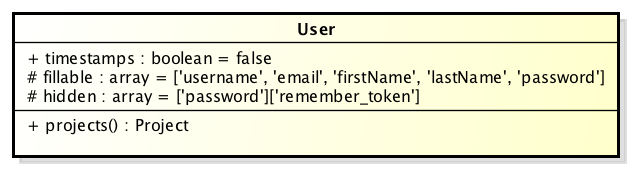
\includegraphics[width=0.7\linewidth]{img/User}
		\caption[Diagramma della classe User]{Diagramma della classe User}
		\label{fig:User}
	\end{figure}

	\subsubsection*{Descrizione}
	Il model User permette di gestire la collection users del database. Eloquent presume che il nome della classe sia il singolare del nome della collection nel database, quindi collega USer alla collection users.
	\subsubsection*{Utilizzo}
	Il model gestisce la collection users del database.
	\subsubsection*{Attributi}
	\begin{itemize}
		\item \textbf{+ timestamps : boolean = false :}\\
		Di default Eloquent automatizza l'inserimento del timestamp relativo all'inserimento e aggiornamento di un campo. Se alla variabile viene assegnato il valore le informazioni dell'inserimento e del aggiornamento non verranno aggiunto alla collection.
		\item \textbf{\# fillable : array = ['username', 'email', 'firstName', 'lastName', 'password']:}\\
		Quando si crea un model, si deve passare una serie di attributi al costruttore del model stesso. Questi attributi vengono assegnati al model tramite \textbf{mass assignment}. La propietà \textit{fillable} serve a specificare quali attributi devono essere assegnabili tramite il mass-assignment.
		\item \textbf{\# hidden : array = ['password', 'remember\_token''] : }\\
		La proprietà hidden si aggiunge quando si vuole limitare gli attributi che sono inclusi nel JSON.
	\end{itemize}
	\subsubsection*{Metodi}
	\begin{itemize}
		\item \textbf{+ projects() : Project}\\
		Abbiamo utilizzato la relazione embedsMany per riuscire ad incorporare il model projects all'interno dell'oggetto principale User. Il metodo ritorna Project su cui verrà chiamato il metodo save() nel caso in cui si voglia aggiornare il modello.
	\end{itemize}
	
\newpage
\subsubsection{Project}

%figura

	\subsubsection*{Descrizione}
	Il model Project rappresenta un progetto creato da un utente. Contiene la presentazio e una o
più infografiche create da esso o nessuna.

	\subsubsection*{Utilizzo}
	Viene utilizzato alla creazione o caricamento di un progetto.
	
	\subsubsection*{Attributi}
	\begin{itemize}
		\item \textbf{+ timestamps : boolean = false :}\\
		Di default Eloquent automatizza l'inserimento del timestamp relativo all'inserimento e aggiornamento di un campo. Se alla variabile viene assegnato il valore le informazioni dell'inserimento e del aggiornamento non verranno aggiunto alla collection.
		\item \textbf{\# fillable : array = [’name’]:}\\
		Quando si crea un model, si deve passare una serie di attributi al costruttore del model stesso. Questi attributi vengono assegnati al model tramite \textbf{mass assignment}. La propietà \textit{fillable} serve a specificare quali attributi devono essere assegnabili tramite il mass-assignment.
		\item \textbf{\# hiddem : array = ['password', 'remember\_token''] : }\\
		La proprietà hidden si aggiunge quando si vuole limitare gli attributi che sono inclusi nel JSON.
	\end{itemize}
	
	\subsubsection*{Metodi}
	\begin{itemize}
		\item \textbf{+ presentation() : Presentation}\\
		Abbiamo utilizzato la relazione embedsOne per riuscire ad incorporare il model Presentation all’interno dell’oggetto principale Project. Il metodo ritorna Presentation su cui verrà chiamato il metodo save() nel caso in cui si voglia aggiornare il modello.
		\item \textbf{+ infographics() : Infographics}\\
		Abbiamo utilizzato la relazione embedsMany per riuscire ad incorporare il model Infographic all’interno dell’oggetto principale Project. Il metodo ritorna Infographic su cui verrà chiamato il metodo save() nel caso in cui si voglia aggiornare il modello.
	\end{itemize}

\newpage
\subsubsection{Infographic}

%figure

	\subsubsection*{Descrizione}
	Questa classe rappresenta un’infografica di un progetto, ovvero una rappresentazione visuale della presentazione per mostrare in maniera semplice e veloce le informazioni.
	
	\subsubsection*{Utilizzo}
Viene utilizzata alla creazione di un’infografica di una presentazione.

\subsubsection*{Attributi}
	\begin{itemize}
		\item \textbf{+ timestamps : boolean = false :}\\
		Di default Eloquent automatizza l'inserimento del timestamp relativo all'inserimento e aggiornamento di un campo. Se alla variabile viene assegnato il valore le informazioni dell'inserimento e del aggiornamento non verranno aggiunto alla collection.
		\item \textbf{\# fillable : array = [’name’, ’path’]:}\\
		Quando si crea un model, si deve passare una serie di attributi al costruttore del model stesso. Questi attributi vengono assegnati al model tramite \textbf{mass assignment}. La propietà \textit{fillable} serve a specificare quali attributi devono essere assegnabili tramite il mass-assignment.
	\end{itemize}


\newpage
\subsubsection{Presentation}

	%figura

	\subsubsection*{Descrizione}
	Questa classe descrive la presentazione di un progetto. Contiene tutte le slide che servono a comporre la presentazione.

	\subsubsection*{Utilizzo}
	Viene utilizzato alla creazione o caricamento di una presentazione.
	
	\subsubsection*{Attributi}
	\begin{itemize}
		\item \textbf{+ timestamps : boolean = false :}\\
		Di default Eloquent automatizza l'inserimento del timestamp relativo all'inserimento e aggiornamento di un campo. Se alla variabile viene assegnato il valore le informazioni dell'inserimento e del aggiornamento non verranno aggiunto alla collection.
		\item \textbf{\# fillable : array = ['title']:}\\
		Quando si crea un model, si deve passare una serie di attributi al costruttore del model stesso. Questi attributi vengono assegnati al model tramite \textbf{mass assignment}. La propietà \textit{fillable} serve a specificare quali attributi devono essere assegnabili tramite il mass-assignment.
	\end{itemize}

	\subsubsection*{Metodi}
	\begin{itemize}
		\item \textbf{+ slides() : Slide}\\
		Abbiamo utilizzato la relazione embedsMany per riuscire ad incorporare il model Slide all’interno dell’oggetto principale Presentation. Il metodo ritorna Slide su cui verrà chiamato il metodo save() nel caso in cui si voglia aggiornare il modello.
	\end{itemize}
\newpage

\subsubsection{Slide}

	%figura

	\subsubsection*{Descrizione}
	Questa classe descrive una singola slide. Contiene tutti i gli oggetti appartenenti alla slide.
	
	\subsubsection*{Utilizzo}
Viene utilizzato alla creazione o caricamento di una slide.

	\subsubsection*{Attributi}
	\begin{itemize}
		\item \textbf{+ timestamps : boolean = false :}\\
		Di default Eloquent automatizza l'inserimento del timestamp relativo all'inserimento e aggiornamento di un campo. Se alla variabile viene assegnato il valore le informazioni dell'inserimento e del aggiornamento non verranno aggiunto alla collection.
		\item \textbf{\# fillable : array = [’xIndex’, ’yIndex']:}\\
		Quando si crea un model, si deve passare una serie di attributi al costruttore del model stesso. Questi attributi vengono assegnati al model tramite \textbf{mass assignment}. La propietà \textit{fillable} serve a specificare quali attributi devono essere assegnabili tramite il mass-assignment.
	\end{itemize}
	\subsubsection*{Metodi}
	\begin{itemize}
		\item \textbf{+ components() : Component}\\
		Abbiamo utilizzato la relazione embedsMany per riuscire ad incorporare il model Component all’interno dell’oggetto principale Slide. Il metodo ritorna Component su cui verrà chiamato il metodo save() nel caso in cui si voglia aggiornare il modello.
	\end{itemize}
\newpage

\subsubsection{Component}

	%figura

	\subsubsection*{Descrizione}
	Questa classe descrive la struttura genera di un componente.
	
	\subsubsection*{Utilizzo}
	Viene utilizzato alla creazione o caricamento di una componente.
	
	\subsubsection*{Attributi}
	\begin{itemize}
		\item \textbf{+ timestamps : boolean = false :}\\
		Di default Eloquent automatizza l'inserimento del timestamp relativo all'inserimento e aggiornamento di un campo. Se alla variabile viene assegnato il valore le informazioni dell'inserimento e del aggiornamento non verranno aggiunto alla collection.
		\item \textbf{\# fillable : array = [’type’, ’originX’, ’OriginY’, ’left’, ’top’, ’width’, ’height’, ’fill’, ’stroke’, ’strokeWidth’, ’strokeDashArray’, ’strokeLineCap’, ’strokeLine-Join’, ’strokeMiterLimit’, ’scaleX’, ’scaleY’, ’angle’, ’flipX’, ’flipY’, ’opacity’, ’shadow’, ’visible’, ’clipTo’, ’backgroundColor’, ’fillRule’, ’globalCompositeOperation']:}\\
		Quando si crea un model, si deve passare una serie di attributi al costruttore del model stesso. Questi attributi vengono assegnati al model tramite \textbf{mass assignment}. La propietà \textit{fillable} serve a specificare quali attributi devono essere assegnabili tramite il mass-assignment.
	\end{itemize}
	

\newpage
\subsubsection{Chart}

%figura

	\subsubsection*{Descrizione}
	Questa classe rappresenta la struttura di dati necessari per descrivere un grafico all’interno di una slide.
	
	\subsubsection*{Utilizzo}
Viene utilizzato alla creazione o caricamento di un grafico.

	\subsubsection*{Attributi}
	\begin{itemize}
		\item \textbf{+ timestamps : boolean = false :}\\
		Di default Eloquent automatizza l'inserimento del timestamp relativo all'inserimento e aggiornamento di un campo. Se alla variabile viene assegnato il valore le informazioni dell'inserimento e del aggiornamento non verranno aggiunto alla collection.
		\item \textbf{\# fillable : array = [’typeChart’ , ’data’]:}\\
		Quando si crea un model, si deve passare una serie di attributi al costruttore del model stesso. Questi attributi vengono assegnati al model tramite \textbf{mass assignment}. La propietà \textit{fillable} serve a specificare quali attributi devono essere assegnabili tramite il mass-assignment.
		
	\end{itemize}
	

\newpage
\subsubsection{RealTimeData}

%figura

	\subsubsection*{Descrizione}
	Questa classe rappresenta la struttura di dati necessari per descrivere RealTimeData (dato in tempo reale) all’interno di una slide.
	
	\subsubsection*{Utilizzo}
	Viene utilizzato alla creazione o caricamento di un RealTimeData.
	
	\subsubsection*{Attributi}
	\begin{itemize}
		\item \textbf{+ timestamps : boolean = false :}\\
		Di default Eloquent automatizza l'inserimento del timestamp relativo all'inserimento e aggiornamento di un campo. Se alla variabile viene assegnato il valore le informazioni dell'inserimento e del aggiornamento non verranno aggiunto alla collection.
		\item \textbf{\# fillable : array = ['pathParser’, ’pathFallback’, ’pathHandlerJs']:}\\
		Quando si crea un model, si deve passare una serie di attributi al costruttore del model stesso. Questi attributi vengono assegnati al model tramite \textbf{mass assignment}. La propietà \textit{fillable} serve a specificare quali attributi devono essere assegnabili tramite il mass-assignment.
		
	\end{itemize}
	
	
\newpage
\subsubsection{Text}

	%figura

	\subsubsection*{Descrizione}
	Questa classe rappresenta la struttura di dati di un campo di testo di una slide.
	
	\subsubsection*{Utilizzo}
	Viene utilizzato alla creazione o caricamento di un campo di testo.
	
	\subsubsection*{Attributi}
	\begin{itemize}
		\item \textbf{+ timestamps : boolean = false :}\\
		Di default Eloquent automatizza l'inserimento del timestamp relativo all'inserimento e aggiornamento di un campo. Se alla variabile viene assegnato il valore le informazioni dell'inserimento e del aggiornamento non verranno aggiunto alla collection.
		\item \textbf{\# fillable : array = [’text’, ’fontSize’, ’fontWeight’, ’fontFamily’, ’fontStyle’, ’lineHeight’, ’textDecoration’, ’textAlign’, ’textBackgroundColor']:}\\
		Quando si crea un model, si deve passare una serie di attributi al costruttore del model stesso. Questi attributi vengono assegnati al model tramite \textbf{mass assignment}. La propietà \textit{fillable} serve a specificare quali attributi devono essere assegnabili tramite il mass-assignment.

	\end{itemize}

\newpage
\subsubsection{Image}

	%figura

	\subsubsection*{Descrizione}
	La classe Image rappresenta la struttura dei dati necessari per rapresentare un’immagine all’interno di una slide.
	
	\subsubsection*{Utilizzo}
	Utilizzata quando viene inserita un’immagine per tenerne traccia.
	
	\subsubsection*{Attributi}
	\begin{itemize}
		\item \textbf{+ timestamps : boolean = false :}\\
		Di default Eloquent automatizza l'inserimento del timestamp relativo all'inserimento e aggiornamento di un campo. Se alla variabile viene assegnato il valore le informazioni dell'inserimento e del aggiornamento non verranno aggiunto alla collection.
		\item \textbf{\# fillable : array = [’src’, ’filters’, ’crossOrigin’, ’alignX’, ’alignY’,’meetOrSlice’, ’background’]:}\\
		Quando si crea un model, si deve passare una serie di attributi al costruttore del model stesso. Questi attributi vengono assegnati al model tramite \textbf{mass assignment}. La propietà \textit{fillable} serve a specificare quali attributi devono essere assegnabili tramite il mass-assignment.

	\end{itemize}

\newpage
\subsubsection{Table}

	%figura

	\subsubsection*{Descrizione}
	Questa classe rappresenta la struttura di dati di una tabella di una slide.
	
	\subsubsection*{Utilizzo}
	Viene utilizzato alla creazione o caricamento di una tabella.
	
	\subsubsection*{Attributi}
	\begin{itemize}
		\item \textbf{+ timestamps : boolean = false :}\\
		Di default Eloquent automatizza l'inserimento del timestamp relativo all'inserimento e aggiornamento di un campo. Se alla variabile viene assegnato il valore le informazioni dell'inserimento e del aggiornamento non verranno aggiunto alla collection.
		\item \textbf{\# fillable : array = [’row’, ’column’, ’title’, ’cellData’]:}\\
		Quando si crea un model, si deve passare una serie di attributi al costruttore del model stesso. Questi attributi vengono assegnati al model tramite \textbf{mass assignment}. La propietà \textit{fillable} serve a specificare quali attributi devono essere assegnabili tramite il mass-assignment.

	\end{itemize}

\newpage
\subsection{Premi::Http::Controllers}
	\begin{figure}[h]
		\centering
		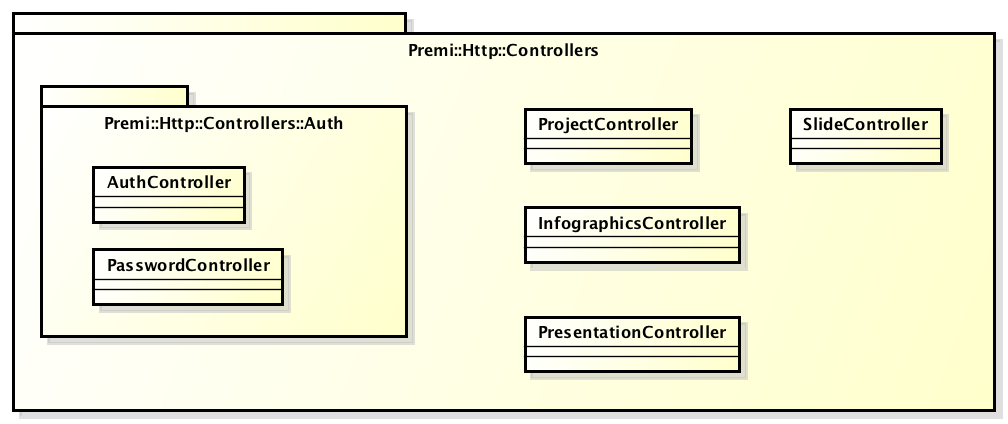
\includegraphics[width=0.7\linewidth]{img/back_end_premi_http_controllers}
		\caption[Premi::Http::Controllers]{Premi::Http::Controllers}
		\label{fig:back_end_premi_http_controllers}
	\end{figure}

I controller accolgono le richieste dal client sfruttando i dati forniti dal model. Attraverso i controller si organizza il comportamento dell'applicazione. Tutti i controller ereditano la classe \textit{Controller} di base incluso nell'installazione di \gls{Laravel}.
\subsubsection{UserController}
\begin{figure}[h]
\centering
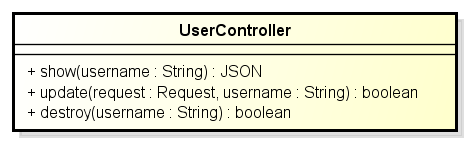
\includegraphics[width=0.8\linewidth]{img/back_end_http_controllers_userController}
\caption[Diagramma della classe UserController]{Diagramma della classe UserController}
\label{fig:back_end_http_controllers_userController}
\end{figure}

	\paragraph{Descrizione}
		Questa classe gestisce i dati dell'utente sfruttando i dati forniti dal model.
	\paragraph{Utilizzo}
		La classe è progettata per consentire l'interrogazione, la manipolazione e l'eliminazione dei dati dell'utente.

	\paragraph{Metodi}
		\begin{itemize}
			\item \textbf{+ show(username: String) : JSON}\\
			Il metodo verifica se c'è un utente autenticato. Se la verifica ha avuto successo si procede con il recupero dei dati dell'utente a cui corrisponde la variabile \textit{username}, in particolare il suo profilo, e restituisce un oggetto JSON contenente tali informazioni:\\
			\textbf{Argomenti}
			\begin{itemize}
				\item username : String;\\
				Stringa contenente il nome utente.
			\end{itemize}
			
			\newpage
			\item \textbf{+ update(request: Request, username: String) : boolean}\\
			Il metodo recupera l'utente autenticato e aggiorna i dati del profilo contenuti nella richiesta HTTP \textit{request}. Il metodo ritorna un valore booleano che indica che i dati sono stati aggiornati:\\
			\textbf{Argomenti}
			\begin{itemize}
				\item request : Request;\\
				Richiesta HTTP contenente i valori con cui eseguire l'aggiornamento del profilo utente.
				\item username : String;\\
				Stringa contenente il nome utente.
			\end{itemize}
			
			\item \textbf{+ destroy(username: String) : boolean}
			Il metodo recupera l'utente autenticato e lo cancella dal database insieme a tutte le  sue informazioni. Il metodo ritorna un valore booleano che indica l'avvenuta cancellazione dal database:\\
			\textbf{Argomenti}
			\begin{itemize}
				\item username : String;\\
				Stringa contenente il nome utente.
			\end{itemize}
		\end{itemize}
		
\newpage
\subsubsection{ProjectController}
\begin{figure}[h]
\centering
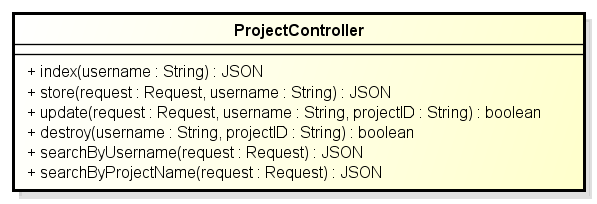
\includegraphics[width=0.8\linewidth]{img/back_end_http_controllers_projectController}
\caption[Diagramma della classe ProjectController]{Diagramma della classe ProjectController}
\label{fig:back_end_http_controllers_projectController}
\end{figure}

	\paragraph{Descrizione}
		Questa classe gestisce i dati di un progetto.
	\paragraph{Utilizzo}
		La classe è progettata per consentire la creazione, la manipolazione dei dati, l'interrogazione e l'eliminazione di un progetto.
		
	\paragraph{Metodi}
		\begin{itemize}
			\item \textbf{+ index(username: String) : JSON}\\
			Il metodo recupera tutti i progetti dell'utente autenticato e li restituisce. Il metodo restituisce un oggetto JSON con le informazioni richieste:\\
			\textbf{Argomenti}
			\begin{itemize}
				\item username : String;\\
				Stringa contenente il nome utente.
			\end{itemize}
			
			\item \textbf{+ store(request: Request, username: String) : boolean}\\
			Il metodo crea un nuovo progetto assegnandoli un nome e lo salva nel database all'interno della collection relativa all'utente autenticato. Il metodo restituisce un oggetto JSON contenente il progetto appena creato. Inoltre emette un segnale di tipo \textit{ProjectWasCreated} per la corretta inizializzazione della presentazione relativa al nuovo progetto:\\
			\textbf{Argomenti}
			\begin{itemize}
				\item request : Request;\\
			 	Richiesta HTTP contenente i valori con cui eseguire la creazione del progetto.
			 	\item username : String;\\
			 	Stringa contenente il nome utente.
			\end{itemize}
			
			\item \textbf{+ update(request: Request, username: String, projectID: String) : boolean}\\
			Il metodo recupera il progetto dell'utente autenticato tramite projectID ed aggiorna i dati del progetto. Il metodo ritorna un valore booleano che indica che l'aggiornamento delle informazioni è avvenuto:\\
			\textbf{Argomenti}
			\begin{itemize}
				\item request : Request;\\
				Richiesta HTTP contenente i valori con cui eseguire l'aggiornamento dei dati del progetto.
				\item username : String;\\
				Stringa contenente il nome utente.
				\item projectID : string; \\
				Stringa contenente l'ID univoco di un progetto.
			\end{itemize}
			
			\item \textbf{+ destroy(username: String, projectID: String) : boolean}\\
			Il metodo recupera il progetto dell'utente autenticato, indicato da projectID, e lo cancella dal database insieme a tutte le sue informazioni. Il metodo ritorna un valore booleano che indica che la cancellazione del progetto dal database è avvenuta:\\
			\textbf{Argomenti}
			\begin{itemize}
				\item username : String;\\
				Stringa contenente il nome utente.
				\item projectID : string; \\
				Stringa contenente l'ID univoco di un progetto.
			\end{itemize}
			
			\item \textbf{+ searchByUsername(request: Request) : JSON}\\
			Il metodo ritorna un oggetto JSON contenente la lista di tutti gli utenti che hanno \textit{username} uguale a quello inserito nell'apposito form:\\
			\textbf{Argomenti}
			\begin{itemize}
				\item request : Request;\\
				Richiesta HTTP contenente il valore con cui effettuare la ricerca.
			\end{itemize}
			
			\item \textbf{+ searchByProjectName(request: Request) : JSON}\\
			Il metodo ritorna un oggetto JSON contenente la lista di tutti i progetti che hanno \textit{name} uguale a quello inserito nell'apposito form:\\
			\textbf{Argomenti}
			\begin{itemize}
				\item request : Request;\\
				Richiesta HTTP contenente il valore con cui effettuare la ricerca.
			\end{itemize}
		\end{itemize}
		
\newpage
\subsubsection{InfographicController}
\begin{figure}[h]
\centering
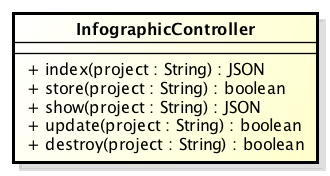
\includegraphics[width=0.8\linewidth]{img/back_end_http_controllers_infographicController}
\caption[Diagramma della classe InfographicController]{Diagramma della classe InfographicController}
\label{fig:back_end_http_controllers_infographicController}
\end{figure}

	\paragraph{Descrizione}
		Questa classe gestisce i dati di un'infografica.
	\paragraph{Utilizzo}
		La classe è progettata per consentire la creazione, la manipolazione dei dati, l'interrogazione e l'eliminazione di un'infografica.
		
	\paragraph{Metodi}
		\begin{itemize}
			\item \textbf{+ index(username: String, projectID: String) : JSON}\\
			Il metodo recupera le infografiche relative ad un progetto dell'utente autenticato e restituisce un oggetto JSON con tutte le infografiche associate al progetto:\\
			\textbf{Argomenti}
			\begin{itemize}
				\item username : String; \\
				Stringa contenente il nome utente.
				\item projectID : String; \\
				Stringa contenente l'ID univoco di un progetto associato all'utente autenticato.
			\end{itemize}
			
			\item \textbf{+ store(request: Request, username: String, projectID: String) : JSON}\\
			Il metodo crea una nuova infografica assegnandoli un nome e il path per il salvataggio e la salva nel progetto con ID = projectID relativo all'utente autenticato. Il metodo ritorna un oggetto JSON contenente l'infografica appena creata:\\
			\textbf{Argomenti}
			\begin{itemize}
				\item request : Request;\\
				Richiesta HTTP contenente i valori con cui creare l'infografica.
				\item username : String; \\
				Stringa contenente il nome utente.
				\item projectID : String; \\
				Stringa contenente l'ID univoco di un progetto associato all'utente autenticato.
			\end{itemize}
			
			\item \textbf{+ show(username: String, projectID: String, infographicID: String) : JSON}\\
			Il metodo interroga il database recuperando il progetto con l'ID = projectID relativo all'utente autenticato ed a partire dal progetto recupera l'infografica con ID = infographicID. Il metodo ritorna un oggetto JSON con le informazioni richieste dell'infografica:\\
			\textbf{Argomenti}
			\begin{itemize}
				\item username : String; \\
				Stringa contenente il nome utente.
				\item projectID : String; \\
				Stringa contenente l'ID univoco di un progetto associato all'utente autenticato.
				\item infographicID : String; \\
				Stringa contenente l'ID univoco di un'infografica associato al progetto.
			\end{itemize}
			
			\item \textbf{+ update(request: Request, username: String, projectID: String, infographicID: String) : boolean}\\
			Il metodo recupera il progetto con ID = projectID relativo all'utente autenticato ed a partire dal progetto recupera l'infografica con ID = infographicID ed aggiorna i dati \textit{name} e \textit{path} dell'infografica. Il metodo ritorna un valore booleano che indica che l'aggiornamento è stato effettuato:\\
			\textbf{Argomenti}
			\begin{itemize}
				\item request : Request;\\
				Richiesta HTTP contenente i valori con cui aggiornare l'infografica.
				\item username : String; \\
				Stringa contenente il nome utente.
				\item projectID : String; \\
				Stringa contenente l'ID univoco di un progetto associato all'utente autenticato.
				\item infographicID : String; \\
				Stringa contenente l'ID univoco di un'infografica associato al progetto.
			\end{itemize}
			
			\item \textbf{+ destroy(username: String, projectID: String, infographicID: String) : boolean}\\
			Il metodo recupera il progetto con ID = projectID relativo all'utente autenticato ed a partire dal progetto recupera l'infografica con ID = infographicID chiamando il metodo \textit{delete} su tale infografica cancellandola dal database. Il metodo ritorna un valore booleano che indica che la cancellazione è avvenuta:\\
			\textbf{Argomenti}
			\begin{itemize}
				\item username : String; \\
				Stringa contenente il nome utente.
				\item projectID : String; \\
				Stringa contenente l'ID univoco di un progetto associato all'utente autenticato.
				\item infographicID : String; \\
				Stringa contenente l'ID univoco di un'infografica associato al progetto.
			\end{itemize}
		\end{itemize}
		
\newpage
\subsubsection{PresentationController}
\begin{figure}[h]
\centering
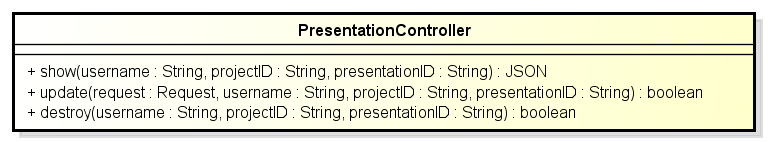
\includegraphics[width=0.8\linewidth]{img/back_end_http_controllers_presentationController}
\caption[Diagramma della classe PresentationController]{Diagramma della classe PresentationController}
\end{figure}


	\paragraph{Descrizione}
		Questa classe gestisce i dati della presentazione.
	\paragraph{Utilizzo}
		La classe è stata progettata per consentire l'interrogazione, la manipolazione dei dati e l'eliminazione di una presentazione.
	
	\paragraph{Metodi}
		\begin{itemize}
			\item \textbf{+ show(username: String, projectID: String, presentationID: String) : JSON}\\
			Il metodo interroga il database recuperando il progetto con l'ID = projectID relativo all'utente autenticato ed a partire dal progetto recupera la presentazione con ID = presentationID. Il metodo ritorna un oggetto JSON con le informazioni richieste della presentazione:\\
			\textbf{Argomenti}
			\begin{itemize}
				\item username : String; \\
				Stringa contenente il nome utente.
				\item projectID : String; \\
				Stringa contenente l'ID univoco di un progetto associato all'utente autenticato.
				\item presentationID : String; \\
				Stringa contenente l'ID univoco della presentazione associata al progetto.
			\end{itemize}
			
			\item \textbf{+ update(request: Request, username: String, projectID: String, presentationID: String) : boolean}\\
			Il metodo recupera il progetto con ID = projectID relativo all'utente autenticato ed a partire dal progetto recupera la presentazione con ID = presentationID ed aggiorna i dati \textit{theme} e \textit{transition} della presentazione. Il metodo ritorna un valore booleano che indica che l'aggiornamento è stato effettuato:\\
			\textbf{Argomenti}
			\begin{itemize}
				\item request : Request;\\
				Richiesta HTTP contenente i valori con cui aggiornare la presentazione.
				\item username : String; \\
				Stringa contenente il nome utente.
				\item projectID : String; \\
				Stringa contenente l'ID univoco di un progetto associato all'utente autenticato.
				\item presentationID : String; \\
				Stringa contenente l'ID univoco di una presentazione associata al progetto.
			\end{itemize}
			\newpage
			\item \textbf{+ destroy(username: String, projectID: String, presentationID: String) : boolean}\\
			Il metodo recupera il progetto con ID = projectID relativo all'utente autenticato ed a partire dal progetto recupera la presentazione con ID = presentationID chiamando il metodo \textit{delete} su tale presentazione cancellandola dal database. Il metodo ritorna un valore booleano che indica che la cancellazione è avvenuta:\\
			\textbf{Argomenti}
			\begin{itemize}
				\item username : String; \\
				Stringa contenente il nome utente.
				\item projectID : String; \\
				Stringa contenente l'ID univoco di un progetto associato all'utente autenticato.
				\item presentationID : String; \\
				Stringa contenente l'ID univoco di una presentazione associata al progetto.
			\end{itemize}
		\end{itemize}
		
\newpage
\subsubsection{SlideController}
\begin{figure}[h]
\centering
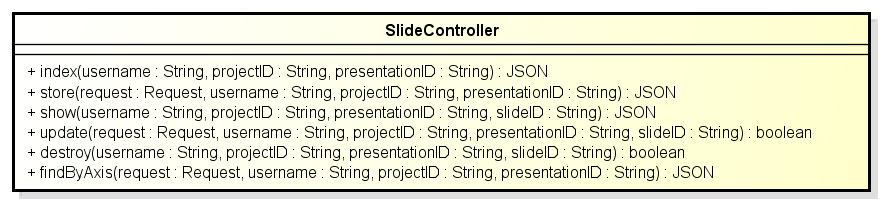
\includegraphics[width=0.8\linewidth]{img/back_end_http_controllers_slideController}
\caption[Diagramma della classe SlideController]{Diagramma della classe SlideController}
\label{fig:back_end_http_controllers_slideController}
\end{figure}

	\paragraph{Descrizione}
		Questa classe gestisce i dati di una slide.
	\paragraph{Utilizzo}
		La classe è stata progettata per consentire la creazione e la manipolazione dei dati di una slide.

	\paragraph{Metodi}
		\begin{itemize}
			\item \textbf{+ index(username: String, projectID: String, presentationID: String) : JSON}\\
				Il metodo recupera il progetto con ID = projectID relativo all'utente autenticato, per poi recuperare l'unica presentazione associata a tale progetto e restituisce tutte le slide associate ad essa. Il metodo ritorna un oggetto JSON contenente le slide all'interno della presentazione:\\
				\textbf{Argomenti:}
				\begin{itemize}
					\item username : String; \\
					Stringa contenente il nome utente.
					\item projectID : String; \\
					Stringa contenente l'ID univoco di un progetto associato all'utente autenticato.
					\item presentationID : String; \\
					Stringa contenente l'ID univoco di una presentazione associata al progetto.
				\end{itemize}
				
			\item \textbf{+ store(request: Request, username: String, projectID: String, presentationID: String) : JSON}\\
				Il metodo crea una nuova slide recuperando il progetto con ID = projectID relativo all'utente autenticato, per poi recuperare l'unica presentazione associata a tale progetto e la slide con ID = slideID. Invoca il metodo statico della classe Presentation \textit{incrementIndex} che aggiorna in modo corretto tutti gli indici delle slide della presentazione. Il metodo ritorna un oggetto JSON che contiene la slide appena creata:\\
				\textbf{Argomenti:}
				\begin{itemize}
					\item request : Request;\\
					Richiesta HTTP contenente i componenti da inserire nella slide.
					\item username : String; \\
					Stringa contenente il nome utente.
					\item projectID : String; \\
					Stringa contenente l'ID univoco di un progetto associato all'utente autenticato.
					\item presentationID : String; \\
					Stringa contenente l'ID univoco di una presentazione associata al progetto.
				\end{itemize}
			
			\newpage
			\item \textbf{+ show(username: String, projectID: String, presentationID: String, slideID: String) : JSON}\\
				Il metodo recupera il progetto con ID = projectID relativo all'utente autenticato, per poi recuperare l'unica presentazione associata a tale progetto e la slide con ID = slideID. Il metodo ritorna un oggetto JSON contenente la slide richiesta:\\
				\textbf{Argomenti:}
					\begin{itemize}
						\item username : String; \\
						Stringa contenente il nome utente.
						\item projectID : String; \\
						Stringa contenente l'ID univoco di un progetto associato all'utente autenticato.
						\item presentationID : String; \\
						Stringa contenente l'ID univoco di una presentazione associata al progetto.
						\item slideID : String; \\
						Stringa contenente l'ID univoco della slide associata alla presentazione.
					\end{itemize}
					
			\item \textbf{+ update(request: Request, username: String, projectID: String, presentationID: String, slideID: String) : b}oolean\\
				Il metodo recupera il progetto con ID = projectID relativo all'utente autenticato, per poi recuperare l'unica presentazione associata a tale progetto e la slide con ID = slideID. Invoca i metodi statici della classe Slide \textit{deleteOldComponents} e \textit{updateNewComponents} per inserire in modo corretto i nuovi componenti passati tramite la richiesta HTTP. Il metodo ritorna un valore booleano che indica che l'aggiornamento è stato effettuato:\\
					\textbf{Argomenti:}
					\begin{itemize}
						\item request : Request;\\
						Richiesta HTTP contenente i componenti con cui aggiornare la slide.
						\item username : String; \\
						Stringa contenente il nome utente.
						\item projectID : String; \\
						Stringa contenente l'ID univoco di un progetto associato all'utente autenticato.
						\item presentationID : String; \\
						Stringa contenente l'ID univoco di una presentazione associata al progetto.
						\item slideID : String; \\
						Stringa contenente l'ID univoco della slide associata alla presentazione.
					\end{itemize}
					
			\item \textbf{+ destroy(username: String, projectID: String, presentationID: String, slideID: String) : boolean}\\
				Il metodo recupera il progetto con ID = projectID relativo all'utente autenticato, per poi recuperare l'unica presentazione associata a tale progetto e la slide con ID = slideID e la elimina dal database cancellando tutte le sue informazioni. Invoca il metodo statico della classe Presentation \textit{decrementIndex} che aggiorna in modo corretto tutti gli indici delle slide della presentazione. il metodo ritorna un valore booleano che indica che la cancellazione nel database è stata effettuata:\\
				\textbf{Argomenti:}
				\begin{itemize}
					\item username : String; \\
					Stringa contenente il nome utente.
					\item projectID : String; \\
					Stringa contenente l'ID univoco di un progetto associato all'utente autenticato.
					\item presentationID : String; \\
					Stringa contenente l'ID univoco di una presentazione associata al progetto.
					\item slideID : String; \\
					Stringa contenente l'ID univoco della slide associata alla presentazione.
				\end{itemize}
				
			\item \textbf{+ findByAxis(request: Request, username: String, projectID: String, presentationID: String) : String}\\
			Il metodo recupera il progetto con ID = projectID relativo all'utente autenticato, per poi recuperare l'unica presentazione associata a tale progetto. Il metodo recupera dalla richiesta HTTP gli indici degli assi X ed Y della slide che si vuole avere, esegue una query per trovare tale slide associata agli indici e ne ritorna l'ID. Ritorna ID = null se non trova nessuna slide:\\
			\textbf{Argomenti:}
			\begin{itemize}
				\item request : Request;\\
				Richiesta HTTP contenente i valori degli assi X ed Y della slide desiderata.
				\item username : String; \\
				Stringa contenente il nome utente.
				\item projectID : String; \\
				Stringa contenente l'ID univoco di un progetto associato all'utente autenticato.
				\item presentationID : String; \\
				Stringa contenente l'ID univoco di una presentazione associata al progetto.
			\end{itemize}
\end{itemize}

\newpage
\subsubsection{Premi::Http::Controllers::Auth}
Laravel implementa un semplice meccanismo di autenticazione. Infatti, quasi tutto è già configurato "out of the box". Il file di configurazione si trova in config/auth.php, che contiene una serie di opzioni, ben documentate, che useremo per ottimizzare il comportamento del servizio di autenticazione.\\
Ognuno di questi controller usa un trait che include i loro metodi necessari.
	\paragraph{AuthController}
	\begin{figure}[h]
\centering
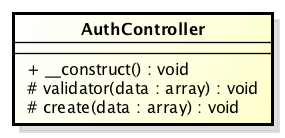
\includegraphics[width=0.5\linewidth]{img/back_end_http_controllers_authController}
\caption[Diagramma della classe AuthController]{Diagramma della classe AuthController}
\label{fig:back_end_http_controllers_authController}
\end{figure}
		\subparagraph{Descrizione}
			AuthController gestisce la registrazione dei nuovi utenti e i loro accessi.
		\subparagraph{Metodi}
			\begin{itemize}
				\item \textbf{+ \_\_construct()}\\
				Il costruttore della classe AuthController.
				\item \textbf{\# validator(data: array) : Validator}\\
				Il metodo si occupa della validazione di tutte le informazioni che riguardano l'utente al momento della registrazione.\\
					\textbf{Argomenti:}
						\begin{itemize}
							\item data : array;
							Array di valori contenente tutti i dati della registrazione di un utente. 
						\end{itemize}
				\item \textbf{\# create(data: array) : User}\\
				Il metodo si occupa della creazione di un nuovo utente:\\
					\textbf{Argomenti:}
						\begin{itemize}
							\item data : array;
							Array di valori contenente tutti i dati della registrazione di un utente.
						\end{itemize}
			\end{itemize}
		
\newpage
	\paragraph{PasswordController}
	\begin{figure}[h]
\centering
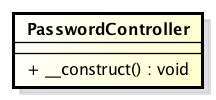
\includegraphics[width=0.5\linewidth]{img/back_end_http_controllers_passwordController}
\caption[Diagramma della classe PasswordController]{Diagramma della classe PasswordController}
\label{fig:back_end_http_controllers_passwordController}
\end{figure}

		\subparagraph{Descrizione}
			PasswordController contiene la logica per aiutare gli utenti per il reset delle loro credenziali di accesso.
		\subparagraph{Metodi}
			\begin{itemize}
				\item \textbf{+ \_\_construct()}\\
				Il costruttore della classe PasswordController.
			\end{itemize}
	

\newpage
\subsection{Premi::Events}
\begin{figure}[h]
	\centering
	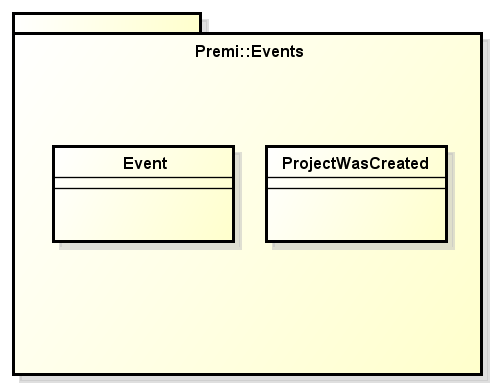
\includegraphics[width=0.7\linewidth]{img/premi_back_end_events}
	\caption[Premi::Events]{Premi::Http::Events}
	\label{fig:premi_back_end_events}
\end{figure}

Gli eventi forniscono una semplice implementazione di osservazione che consente all'applicazione di restare in ascolto di eventuali eventi lanciati da qualche funzione.
\subsubsection{Event}
\begin{figure}[h]
	\centering
	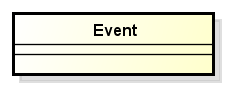
\includegraphics[width=0.5\linewidth]{img/premi_back_end_event}
	\caption[Diagramma della classe Event]{Diagramma della classe Event}
	\label{fig:premi_back_end_event}
\end{figure}


\paragraph{Descrizione}
La classe Events è una classe astratta che viene estesa da tutti i nuovi eventi creati.

\newpage
\subsubsection{ProjectWasCreated}
\begin{figure}[h]
	\centering
	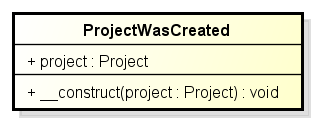
\includegraphics[width=0.5\linewidth]{img/premi_back_end_project_was_created}
	\caption[Diagramma della classe ProjectWasCreated]{Diagramma della classe ProjectWasCreated}
	\label{fig:premi_back_end_project_was_created}
\end{figure}


\paragraph{Descrizione}
La classe ProjectWasCreated è un evento che gestisce la creazione di un nuovo progetto, creando una presentazione con prima \gls{slide} di default ad esso correlato.

\paragraph{Utilizzo}
Utilizzata quando viene creato un nuovo progetto.

\paragraph{Attributi}
\begin{itemize}
	\item \textbf{+ project : Project}\\
	Variabile di istanza che contiene il progetto che ha generato l'evento.   
\end{itemize}

\paragraph{Metodi:}
\begin{itemize}
	\item \textbf{+ \_\_construct(project: Project) : void}\\
	Crea una nuova istanza dell'evento:\\
	\textbf{Argomenti:}
	\begin{itemize}
		\item project : Project;
		Progetto che ha scatenato l'evento.
	\end{itemize}
\end{itemize}


\newpage
\subsection{Premi::Listeners}
\begin{figure}[h]
	\centering
	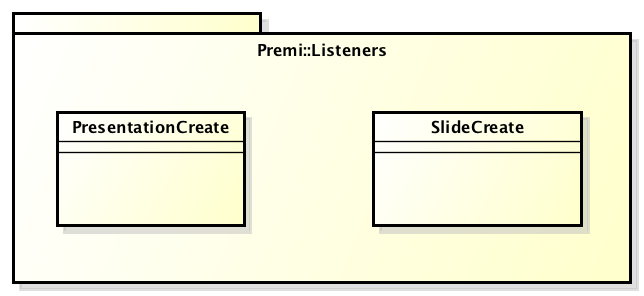
\includegraphics[width=0.7\linewidth]{img/back_end_premi_listeners}
	\caption[Premi::Http::Listeners]{Premi::Http::Listeners}
	\label{fig:back_end_premi_listeners}
\end{figure}

I listeners restano in ascolto, in attesa di essere chiamati da qualche evento, e contengono al loro interno la logica per rispondere  all'evento che li ha invocati. 
\subsubsection{PresentationCreate}
\begin{figure}[h]
	\centering
	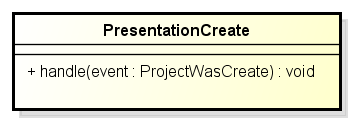
\includegraphics[width=0.5\linewidth]{img/premi_back_end_presentation_create}
	\caption[Diagramma della classe PresentationCreate]{Diagramma della classe PresentationCreate}
	\label{fig:premi_back_end_presentation_create}
\end{figure}


\paragraph{Descrizione}
La classe PresentationCreate risponde all'evento ProjectWasCreate e crea una presentazione associata al progetto appena creato.

\paragraph{Utilizzo}
Utilizzata quando viene creato un nuovo progetto e lanciato l'evento ProjectWasCreated.

\paragraph{Metodi:}
\begin{itemize}
	\item \textbf{+ handle(event: ProjectWasCreated) : void}\\
	Crea una nuova presentazione associata al progetto contenuto, e che ha invocato, l'evento ProjectWasCreated:\\
	\textbf{Argomenti:}
	\begin{itemize}
		\item project : Project;
		L'evento che ha chiamato il listener.
	\end{itemize}
\end{itemize}

\subsubsection{SlideCreate}
\begin{figure}[h]
	\centering
	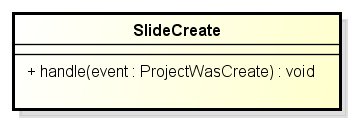
\includegraphics[width=0.5\linewidth]{img/premi_back_end_slide_create}
	\caption[Diagramma della classe SlideCreate]{Diagramma della classe SlideCreate}
	\label{fig:premi_back_end_slide_create}
\end{figure}


\paragraph{Descrizione}
La classe SlidCreate risponde all'evento ProjectWasCreate e crea una prima slide di default all'interno della presentazione associata al progetto appena creato.

\paragraph{Utilizzo}
Utilizzata quando viene creato un nuovo progetto e lanciato l'evento ProjectWasCreated.

\paragraph{Metodi:}
\begin{itemize}
	\item \textbf{+ handle(event: ProjectWasCreated) : void}\\
	Crea una prima slide di default della presentazione associata al progetto contenuto, e che ha invocato, l'evento ProjectWasCreated:\\
	\textbf{Argomenti:}
	\begin{itemize}
		\item project : Project;
		L'evento che ha chiamato il listener.
	\end{itemize}
\end{itemize}
